\documentclass[11pt]{article} % use larger type; default would be 10pt

\usepackage{graphicx} % support the \includegraphics command and options
\usepackage{amsmath}
\usepackage{fullpage}
\usepackage[center]{caption}

\title{Stochastic Collocation}
\author{Paul Talbot}
%\date{} % Activate to display a given date or no date (if empty),
         % otherwise the current date is printed 

\begin{document}
\maketitle

\section{Introduction}
The concept behind using stochastic collocation for propagating uncertainty is that the uncertainty space can be spanned by quadrature rules deterministically instead of using stochastic sampling.

\section{Uncertainty}
TODO -realizations
\subsection{Uncertain Variables}
We consider a given variable $x$ with some uncertainty in value.  We define $\bar x$ as the average value of this variable.  The uncertainty in $x$ can be given in several ways.  In this work we consider two types of uncertainty: uniform and normal.
\subsubsection{Uniformly-Uncertain Variables}
A uniformly-uncertain variable, hereafter referred to as uniform variable, has an equal probability of being realized at all its potential values.  For example, for a six-sided die, each face is equally probable to end facing up when the die is rolled.  For a continuous uniform variable, the range of realizations are well-described by an average value $\bar x$, minimum value $\bar x -\sigma$, and maximum value $\bar x+\sigma$.  We note the following characteristics of uniform variables:
\begin{itemize}
\item The possible values of $x$ range linearly from $\bar x-\sigma$ to $\bar x+\sigma$.
\item The possible values of $x$ as a function of $w$ are found along $x(w)=\sigma w+\bar x$.
\item The probability of any realization $w$ is given by a horizontal distribution $P(w)$ which has a value of $1/2$ from $-$1 to 1 and is zero everywhere else.
\end{itemize}
\begin{figure}[h!]
\centering
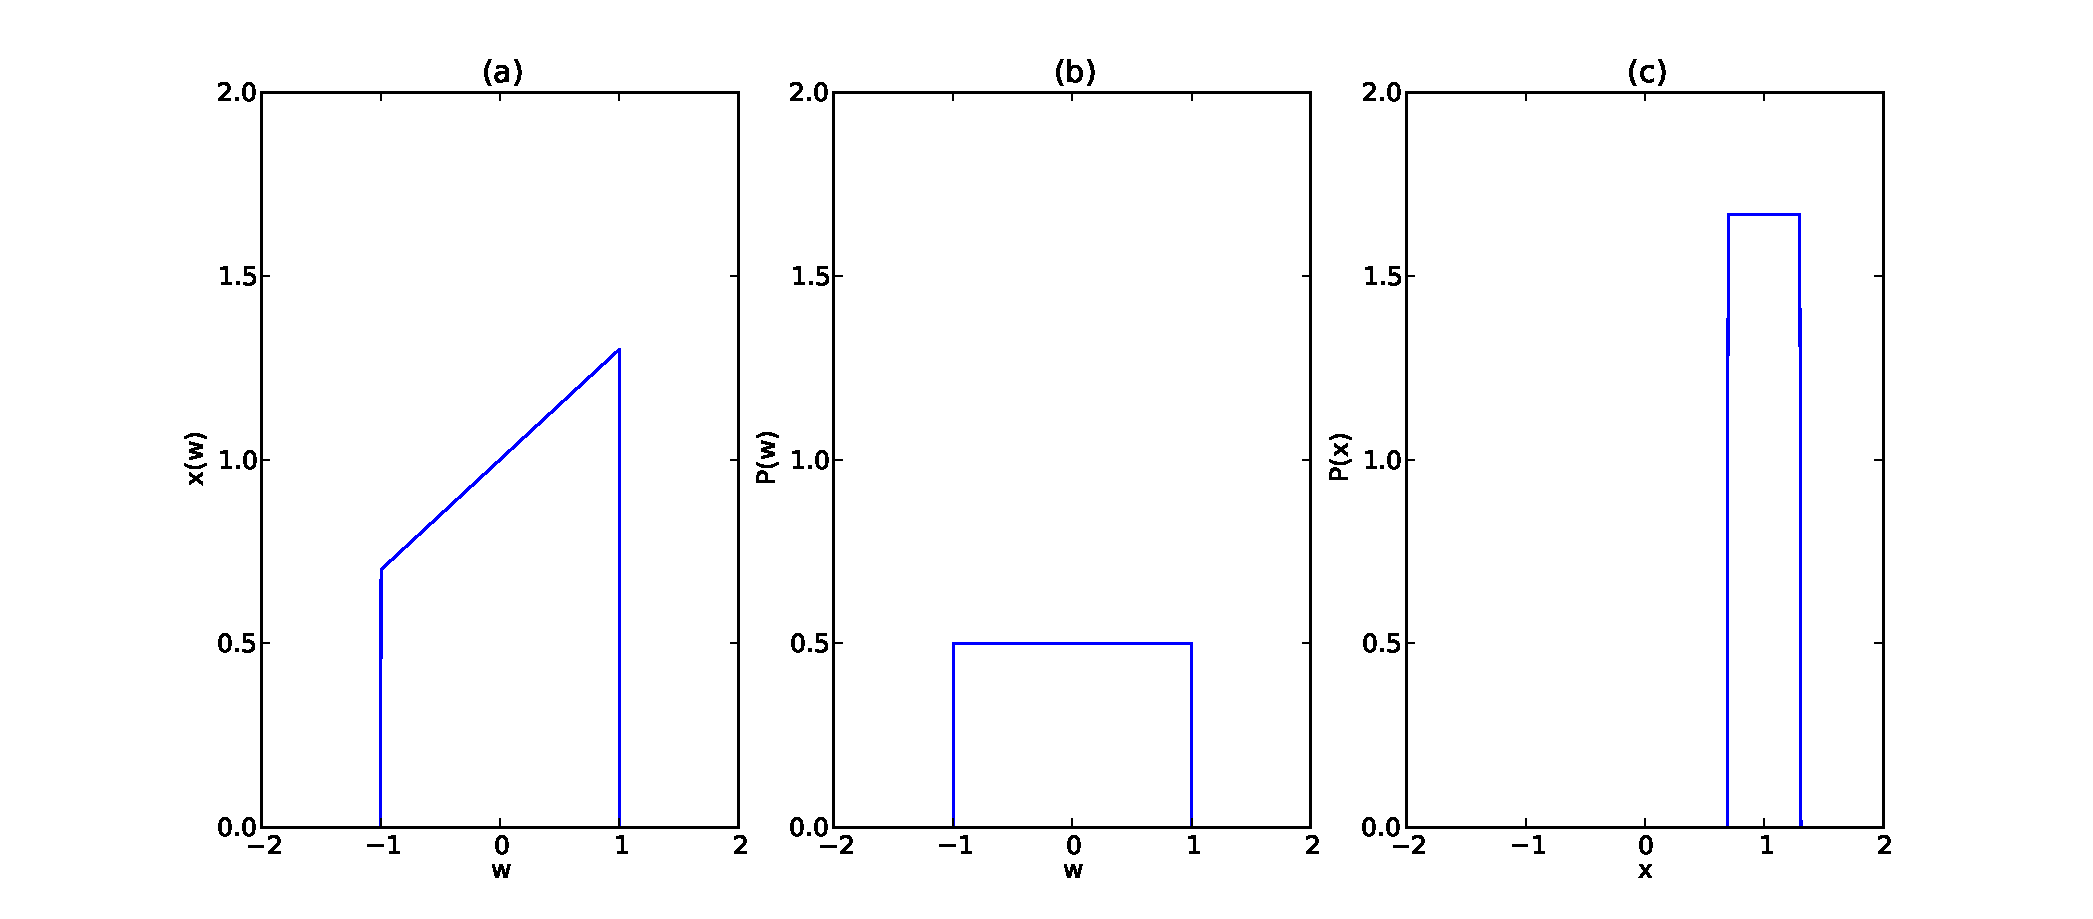
\includegraphics[width=\linewidth]{figUniVar}
\label{figUniVar}
\caption{(a) Possible values of $x(w)$ as a function of $w$. (b) Probability distribution of $w$. \newline(c) Probability distribution of $x(w)$.}
\end{figure}

\subsection{Uncertain Processes}
TODO



\section{Quadrature}
Gaussian quadrature makes the following assumption:
\begin{equation}
  \int_a^b f(x)dx=\int_a^b g(x) P(x)dx\approx\sum_n^N w_n f(x_n),
\end{equation}
where $f(x)$ is any function continuous over the interval $a\to b$, $P(x)$ is a probability distribution function for $x$, $N$ is the order of quadrature chosen and $w_n$ and $x_n$ are given by the choice of quadrature and its order.  In general $x_n$ are referred to as the abscissas of the quadrature, and $w_n$ as the associated weights.  In the limit that $N$ approaches infinity, the quadrature is exact. 

There are many different Gaussian quadrature sets that may are selected based on their abscissa distribution and the limits $a$ and $b$ of the integral in question.

\subsection{Implementing Integration with Quadrature}
Here we pause to make a note of the methods surrounding evaluating integrals using quadrature sets.  We consider in particular an implemented function \texttt{integrate(f(x))} that accepts a function and integrates it using quadrature.  In general, as above, a quadrature evaluates an integral using some weighting function $P(x)$, not to be confused with the quadrature weights $w_n$.  The Legendre quadrature is singular because its weighting function is 1; this means that $f(x)=g(x)$ for Legendre quadrature, and a function \texttt{integrateLegendre(f(x))} that uses Legendre quadrature will integrate $f(x)$ exactly as expected.

For other quadrature sets, however, $P(x)\neq 1$ and a function such as \texttt{integrateHermite(f(x))} will not accurately return $\int f(x) dx$.  Use of these quadrature sets require some knowledge of the user, since the integration routine will actually integrate $\int f(x) P(x)dx$.  In the case of Hermite quadrature, $P(x)=\exp(-x^2)$, so \texttt{integrateHermite(f(x))} would return $\int f(x)\exp(-x^2) dx$.  This is useful for a user that wants to integrate a function times a weighting factor by only passing the function.

\subsection{Gauss-Legendre}
Gauss-Legendre quadrature spans $[-1,1]$ with $P(x)=1$, and is perhaps the most commonly used quadrature in particle transport.  The abscissa are given by finding the roots of the Legendre polynomials
\begin{equation}
P_N(x)=\frac{1}{2^NN!}\frac{d^N}{dx^N}[(x^2-1)^N],
\end{equation}
and the weights are given by
\begin{equation}
w_n=\frac{2}{(1-x_n^2)[P'_N(x_n)]^2}.
\end{equation}
Gauss-Legendre quadrature is well-suited for spanning the uncertainty space of uniformly-distributed uncertainty.


\subsection{Gauss-Hermite}
Gauss-Hermite quadrature spans $[-\infty,\infty]$ and $W(x)=e^{-x^2}$.  The abscissa come from the roots of the physicist's Hermite polynomial
\begin{equation}
H_N(x)=(-1)^Ne^{x^2}\frac{d^N}{dx^N}e^{-x^2},
\end{equation}
and the weights are given by
\begin{equation}
w_n=\frac{2^{N-1}N!\sqrt\pi}{N^2[H_{N-1}(x_n)]^2}.
\end{equation}
Gauss-Hermite quadrature is well-suited for spanning the uncertainty space of normally-distributed uncertainty; however, careful consideration must be made of the probability function associated with choosing the Hermite quadrature.  Since we are most interested in using Hermite quadrature to span the uncertainty space of a variable with normal (Gaussian)-distributed uncertainty, we desire the probability distribution to be normal; that is, we desire the probability distribution to be $P(x)=e^{-x^2/2}$, noting the half in the numerator.  We can adjust our integral to agree well with the normal distribution probability function by defining
\begin{equation}
b\equiv\frac{a}{\sqrt{2}},\hspace{20pt}a=\sqrt{2}b.
\end{equation}
The integral we desire to approximate using the normal distribution is
\begin{equation}
\frac{1}{\sqrt{2\pi}}\int_{-\infty}^{\infty} f(a)e^{a^2/2}da\approx\sum_iw_if(a_i).
\end{equation}
Replacing $b\sqrt{2}$ for $a$ everywhere restores the Hermite form of the integral,
\begin{equation}
\frac{1}{\sqrt{2\pi}}\int_{-\infty}^{\infty} f(b\sqrt{2})e^{b^2}\sqrt{2}db\approx\sum_i\frac{w_i}{\sqrt\pi}f(b_i\sqrt{2}).
\end{equation}
\end{document}
